
\section{Wednesday}\index{Wednesday_lecture}
\subsection{Laplace Transformation}
\[\lapl{f}(s)=\int_0^\infty e^{-st}f(t)\diff t
\]
\[|f(t)\leq Me^{ct}|\qquad\text{for t large, } s>c
\]
Heariside function $H(t)$
\begin{figure}[H]
\centering
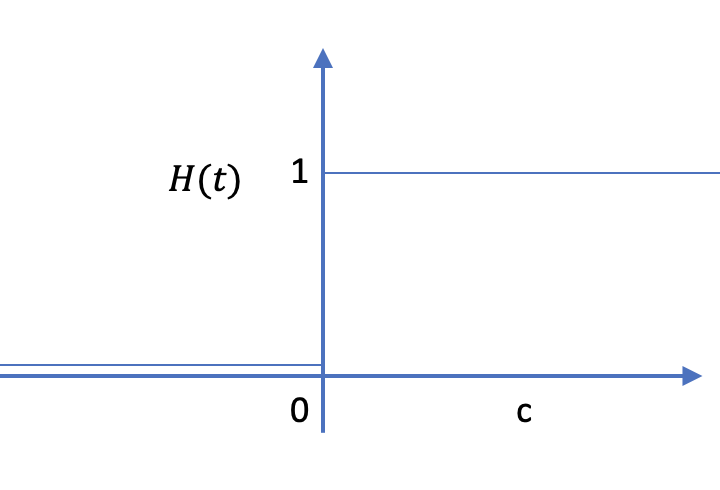
\includegraphics[width=6cm]{week9_1}
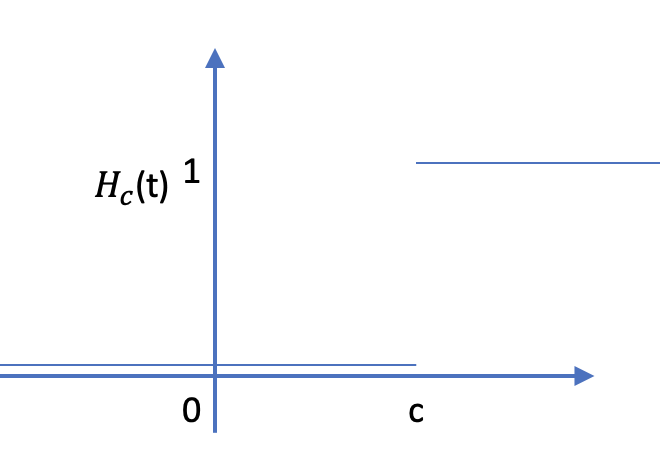
\includegraphics[width=6cm]{week9_2}
\end{figure}

\paragraph{lemma}
\[\lapl{H_c(t)f(t-c)}(s)=e^{-cs}F(s)\]
($F(s)=\lapl{f}(s)$)
\begin{figure}[H]
\centering
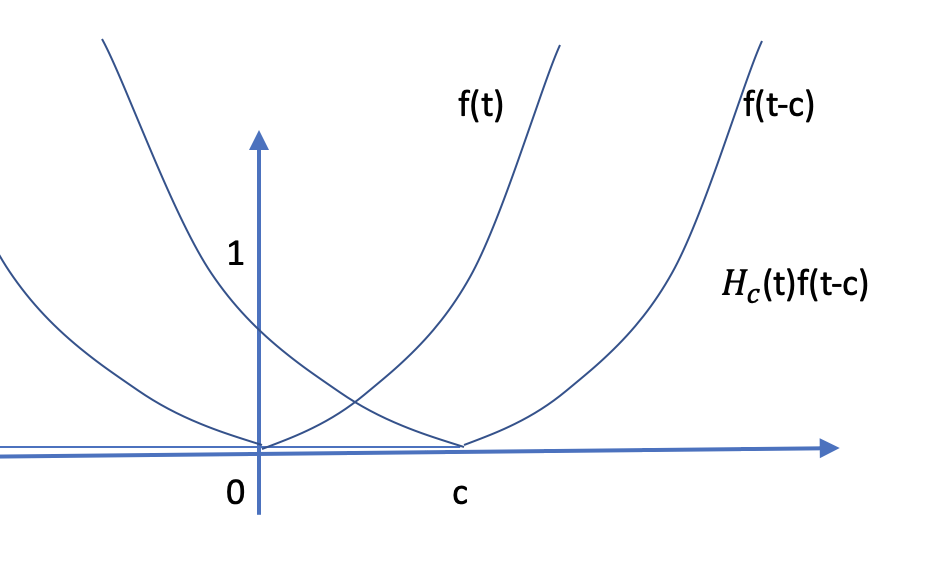
\includegraphics[width=8cm]{week9_3}
\end{figure}
\begin{proof}
\[\begin{aligned}
&\lapl{H_c(t)f(t-c)}(s)\\
=&\int_0^\infty e^{-st}H_c(t)f(t-c)\diff t\\
=&\int_c^\infty e^{-st}f(t-c)\diff t
\end{aligned}\]
$\bar{t}=t-c$
\[=\int_0^\infty e^{-s(\bar{t}+c)}f(\bar{t})\diff \bar{t}
\]
\[=\int_0^\infty e^{-s\bar{t}}f(\bar{t})\diff \bar{t} e^{-sc}
\]
\[=\lapl{f}(s)e^{-sc}
\]
\end{proof}
\begin{example}
\[y\pp-3y\p+2y=\begin{cases}\frac{1}{c},\quad 1<t<1+c\\0, \text{otherwise}\end{cases}
\]
\begin{figure}[H]
\centering
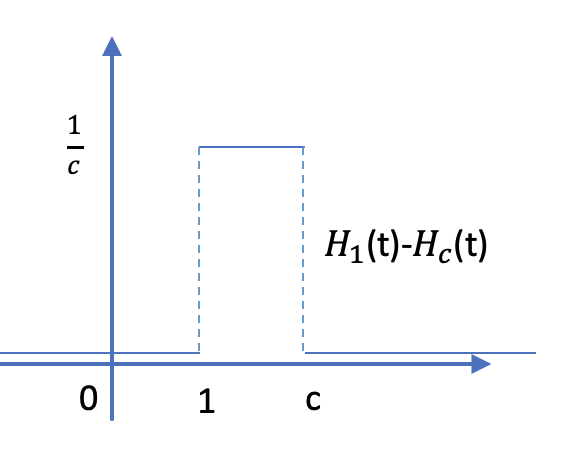
\includegraphics[width=6cm]{week9_4}
\end{figure}
\[Y=\lapl{y}\qquad y(0)=y\p(0)=0
\]
\[\begin{aligned}
&\lapl{y\pp-3y\p+2y}(s)\\
=&s^2Y(s)-3sY(s)+2Y(s)\\
=&Y(s)(s^2-3s+2)\dots(1)
\end{aligned}
\]
\[\begin{aligned}\lapl{\frac{1}{c}[H_1(t)-H_{1+c}(t)]}(s)&=\frac{1}{c}(\lapl{H_1(t)}(s)-\lapl{H_{1+c}(t)}(s))\\&=\frac{1}{c}(\frac{e^{-s}}{s}-\frac{e^{-(1+c)s}}{s})\dots(2)\end{aligned}
\]
(1)=(2), as we take laplace transformation on both side of the given equation in this example.
\[\begin{aligned}\therefore Y(s)&=\frac{\frac{1}{c}e^{-s}(1-e^{-cs})}{(s-1)(s-2)s}\\
&=\frac{1}{c}e^{-s}(1-e^{-cs})[\frac{1}{2s}-\frac{1}{s-1}+\frac{1}{2}\frac{1}{s-2}]\dots(3)\\
&=\frac{1}{c}e^{-s}(1-e^{-cs})\lapl{\frac{1}{2}-e^t+\frac{1}{2}e^{2t}}\dots(4)\\
&=\frac{1}{c}\lapl{H_1(t)[\frac{1}{2}-e^{t-1}+\frac{1}{2}e^{2(t-1)}]-H_{1+c}[\frac{1}{2}-e^{t-1-c}+\frac{1}{2}e^{2(t-1-c)}]}\dots(5)
\end{aligned}
\]
From (3) to (4), we do reverse laplace transformation, such as $\lapl{1}(s)=\int_0^\infty e^{-st}1\diff t=\dots=\frac{1}{s}$ and $\lapl{H_1(t)}(s)=e^{-s}\lapl{1}(s)$ (lemma above).\\
Procedure from (4) to (5) is due to lemma above.\\
Remember $Y(s)=\lapl{y}$
\[\begin{aligned}y(t)&=\frac{1}{c}\{H_1(t)[\frac{1}{2}-e^{t-1}+\frac{1}{2}e^{2(t-1)}]-H_{1+c}[\frac{1}{2}-e^{t-1-c}+\frac{1}{2}e^{2(t-1-c)}]\}\\
&=\frac{1}{c}\begin{cases}0,~t\leq1\\\frac{1}{2}-e^{t-1}+\frac{1}{2}e^{2(t-1)},~1<t<1+c\\-e^{t-1}+\frac{1}{2}e^{2(t-1)}+e^{t-1-c}-\frac{1}{2}e^{2(t-1-c)},~t\geq1+c\end{cases}
\end{aligned}
\]
As $c\rightarrow0$, $\frac{1}{2}e^{2(t-1)}\frac{1-e^{-2c}}{c}-e^{t-1}\frac{1-e^{-c}}{c}\rightarrow e^{2(t-1)}-e^{t-1}$ (by L'hospital's rule).

\end{example}

There is another way of doing this problem.
\begin{definition}[``Delta'' function: $\delta$] For any smooth function $\varphi$ with compact support on $\mathbb{R}$
\[\int_{-\infty}^\infty \delta(t)\varphi(t)\diff t=\varphi(0)
\]\end{definition}
\begin{example}[Example of delta function: ``Approximation to identity'']
A sequence of functions $\{\eta_\varepsilon\}$, $\eta(x)$ smooth supported inside $(-1,1)$, $\eta(-x)=\eta(x)\geq0$ and $\int_{-1}^1\eta(x)\diff x=1$\\
\[\eta(x)=\begin{cases}ce^{-\frac{1}{1-x^2}}~~|x|\leq1\\0~~|x|\geq1\end{cases}
\]
$c$ is chosen such that $\int_{-1}^1\eta=1$.
\[\eta_\varepsilon=\frac{1}{\varepsilon}\eta(\frac{x}{\varepsilon})
\]
 Want to show $\lim_{\varepsilon\rightarrow0}\eta_\varepsilon=\delta$, i.e. $\lim_{\varepsilon\rightarrow0}\int_{-\infty}^\infty\eta_\varepsilon(x)\varphi(x)\diff x=\varphi(0)$.
\end{example}
\begin{proof}
\[\int_{-\infty}^\infty\eta_\varepsilon(x)\diff x=1
\]
\[\begin{aligned}
|\int_{-\infty}^\infty\eta_\varepsilon(x)\varphi(x)\diff x-\varphi(0)|&=|\int_{-\infty}^\infty\eta_\varepsilon(x)\varphi(x)\diff x-\int_{-\infty}^\infty\eta_\varepsilon(x)\varphi(0)\diff x|\\
&\leq\int_{-\infty}^\infty|\eta_\varepsilon(x)[\varphi(x)-\varphi(0)]|\diff x=\int_{-\varepsilon}^\varepsilon\eta_\varepsilon(x)|\varphi(x)-\varphi(0)|\diff x\\
&\leq\int_{-\varepsilon}^\varepsilon\eta_{\varepsilon}(x)\diff x|\max_{|x|\leq\varepsilon}|\varphi(x)-\varphi(0)||\rightarrow0
\end{aligned}
\]




\end{proof}
\begin{remark}
Delta function isn't a function. As $\delta=\lim_{\varepsilon\rightarrow0}\eta_\varepsilon$, we can see delta function doesn't satisfy the definition of function at point 0. \\
In addition, the integral of delta function is equal to 1.

\end{remark}
\begin{example}
\[y\pp-3y\p+2y=\begin{cases}\frac{1}{c},~1<t<1+c\\0,~ \text{othrwise}\end{cases}
\]
\[y(0)=y\p(0)=0
\]
When $c\rightarrow0$, this question is the same as solve 
\[y\pp-3y\p+2y=\delta(t-1)
\]
\[Y(s)(s^2-3s+2)=\lapl{\delta(t-1)}(s)=\int_0^\infty e^{-st}\delta(t-1)\diff t
\]
\[\begin{aligned}
\therefore Y(s)&=\frac{e^{-s}}{(s-1)(s-2)}\\
&=e^{-s}(\frac{-1}{s-1}+\frac{1}{s-2})\\
&=\lapl{H_1(t)e^{t-1}+H_1(t)e^{2(t-1)}}(s)\\
&=\begin{cases}0,~t\leq1\\e^{2(t-1)}-e^{ct-1},~t\geq1\end{cases}
\end{aligned}
\]




\end{example}











